\documentclass[a4paper,german]{article}
%%BeginIpePreamble

\usepackage{amsmath}
\usepackage{amssymb}
% % Deutsche Silbentrennung
% \usepackage[ngerman]{babel}
% % Deutsche Umlaute
% \usepackage[ansinew]{inputenc}
% %\usepackage[latin1]{inputenc}
\usepackage{graphicx}
\usepackage{xspace}
\usepackage{eurosym}
%Binds \euro to some version of the Euro Symbol

 
\setlength{\parindent}{0pt}
\setlength{\parskip}{3pt}

% editing
\newcommand{\itbox}[1]{\mbox{\it #1\/}}
%\newcommand{\itbox}[1]{\mathit{#1}}
\newcommand{\abbrev}[1]{{\small #1}}
% Starts a new line nearly everywhere
\newcommand{\nl}{\mbox{}\\}
\newcommand{\nlskip}[1]{\mbox{}\\[#1]}
\newcommand{\eod}{\rule{\textwidth}{1pt}\nl \textit{End of Document}}

%Uncertain items
\newcommand{\qq}[1]{?`#1?}

%
%Comments
\newcommand{\cncpt}[1]{\framebox{#1}}
\newcommand{\bgcncpt}[1]{\nl\framebox{\parbox{.95\textwidth}{#1}}\nl[2mm]}
%\renewcommand{\bigconcept}[1]{}
%
%Around formulas
\newcommand{\punctsep}{\hspace{.5ex}}

%%%%%%%%%%%%%%%%%%%%%%%%%%%%%%%%%%%%%%%%%%%%%%%%%%%%%%%%%%%%%%%%%%%%%%%%%%

% Date of writing
\newcommand{\creationDateA}{150130}
% \newcommand{\creationDateB}{150130}
% \newcommand{\creationDateC}{JJMMTT}

% event name (part of file name)
\newcommand{\eventDescription}{VnVDmnstrtnCncpt}

% Version number (part of file name)
\newcommand{\versionNumber}{01}

% Start date of meeting
\newcommand{\meetingStartDate}{\creationDateA}
\newcommand{\meetingStartTime}{10:00}
% End date of meeting
\newcommand{\meetingEndDate}{\meetingStartDate}
\newcommand{\meetingEndTime}{16:30}

%%%%%%%%%%%%%%%%%%%%%%%%%%%%%%%%%%%%%%%%%%%%%%%%%%%%%%%%%%%%%%%%%%%%%%%%%%

\begin{document}
\title{Concept for Demonstration of (some) Verification and Validation
at the ITEA Review March 2015}
\author{Hardi Hungar}
\date{Version \versionNumber, 20\creationDateA}

%\pagestyle{empty}

\maketitle
%
\begin{abstract} 

\end{abstract}

\section*{Document Control}

\begin{tabular}{|l|r|*{2}{p{.3\textwidth}|}}
\hline
\multicolumn{4}{|l|}{\texttt{PR\_TS\_\eventDescription\_\creationDateA\_\versionNumber.tex}}
\\\hline
\textbf{Version} & \textbf{Date} & \textbf{Changes} & \textbf{Comment}
\\\hline
01 & \creationDateA & All sections & Initial 
\\\hline
\end{tabular}



\section{Verification of the WP3 ``First Iteration'' Release}
\label{sec:firstIteration}

\paragraph{Terminology (here)}
\begin{description}
\item[Release] The full SCADE model (executable) in the release
\item[Component] A component (sub-model) contained the \textbf{Release} 
\end{description}


This concept contains some proposals how to demonstrate some VnV on
the \textbf{model}. Part of it is to be performed by the DLR. It
concept presents \emph{some} activities, it is not meant to be
comprehensive. I.e., there may be other activities.

Here, it is assumed that the openETCS development process is a rather
ordinary instantiation of the illustrative development process No.~2
of the EN~50128 (to be described in a revision/elaboration of
D2.3). The \textbf{Release} is considered as part of a
\textit{Detailed SW Design} of the OBU. This would have to be verified
against the artifacts from a proevious design step, the \textit{SW
  Architecture and Design}.

\begin{figure}[hbt]
  \centering
  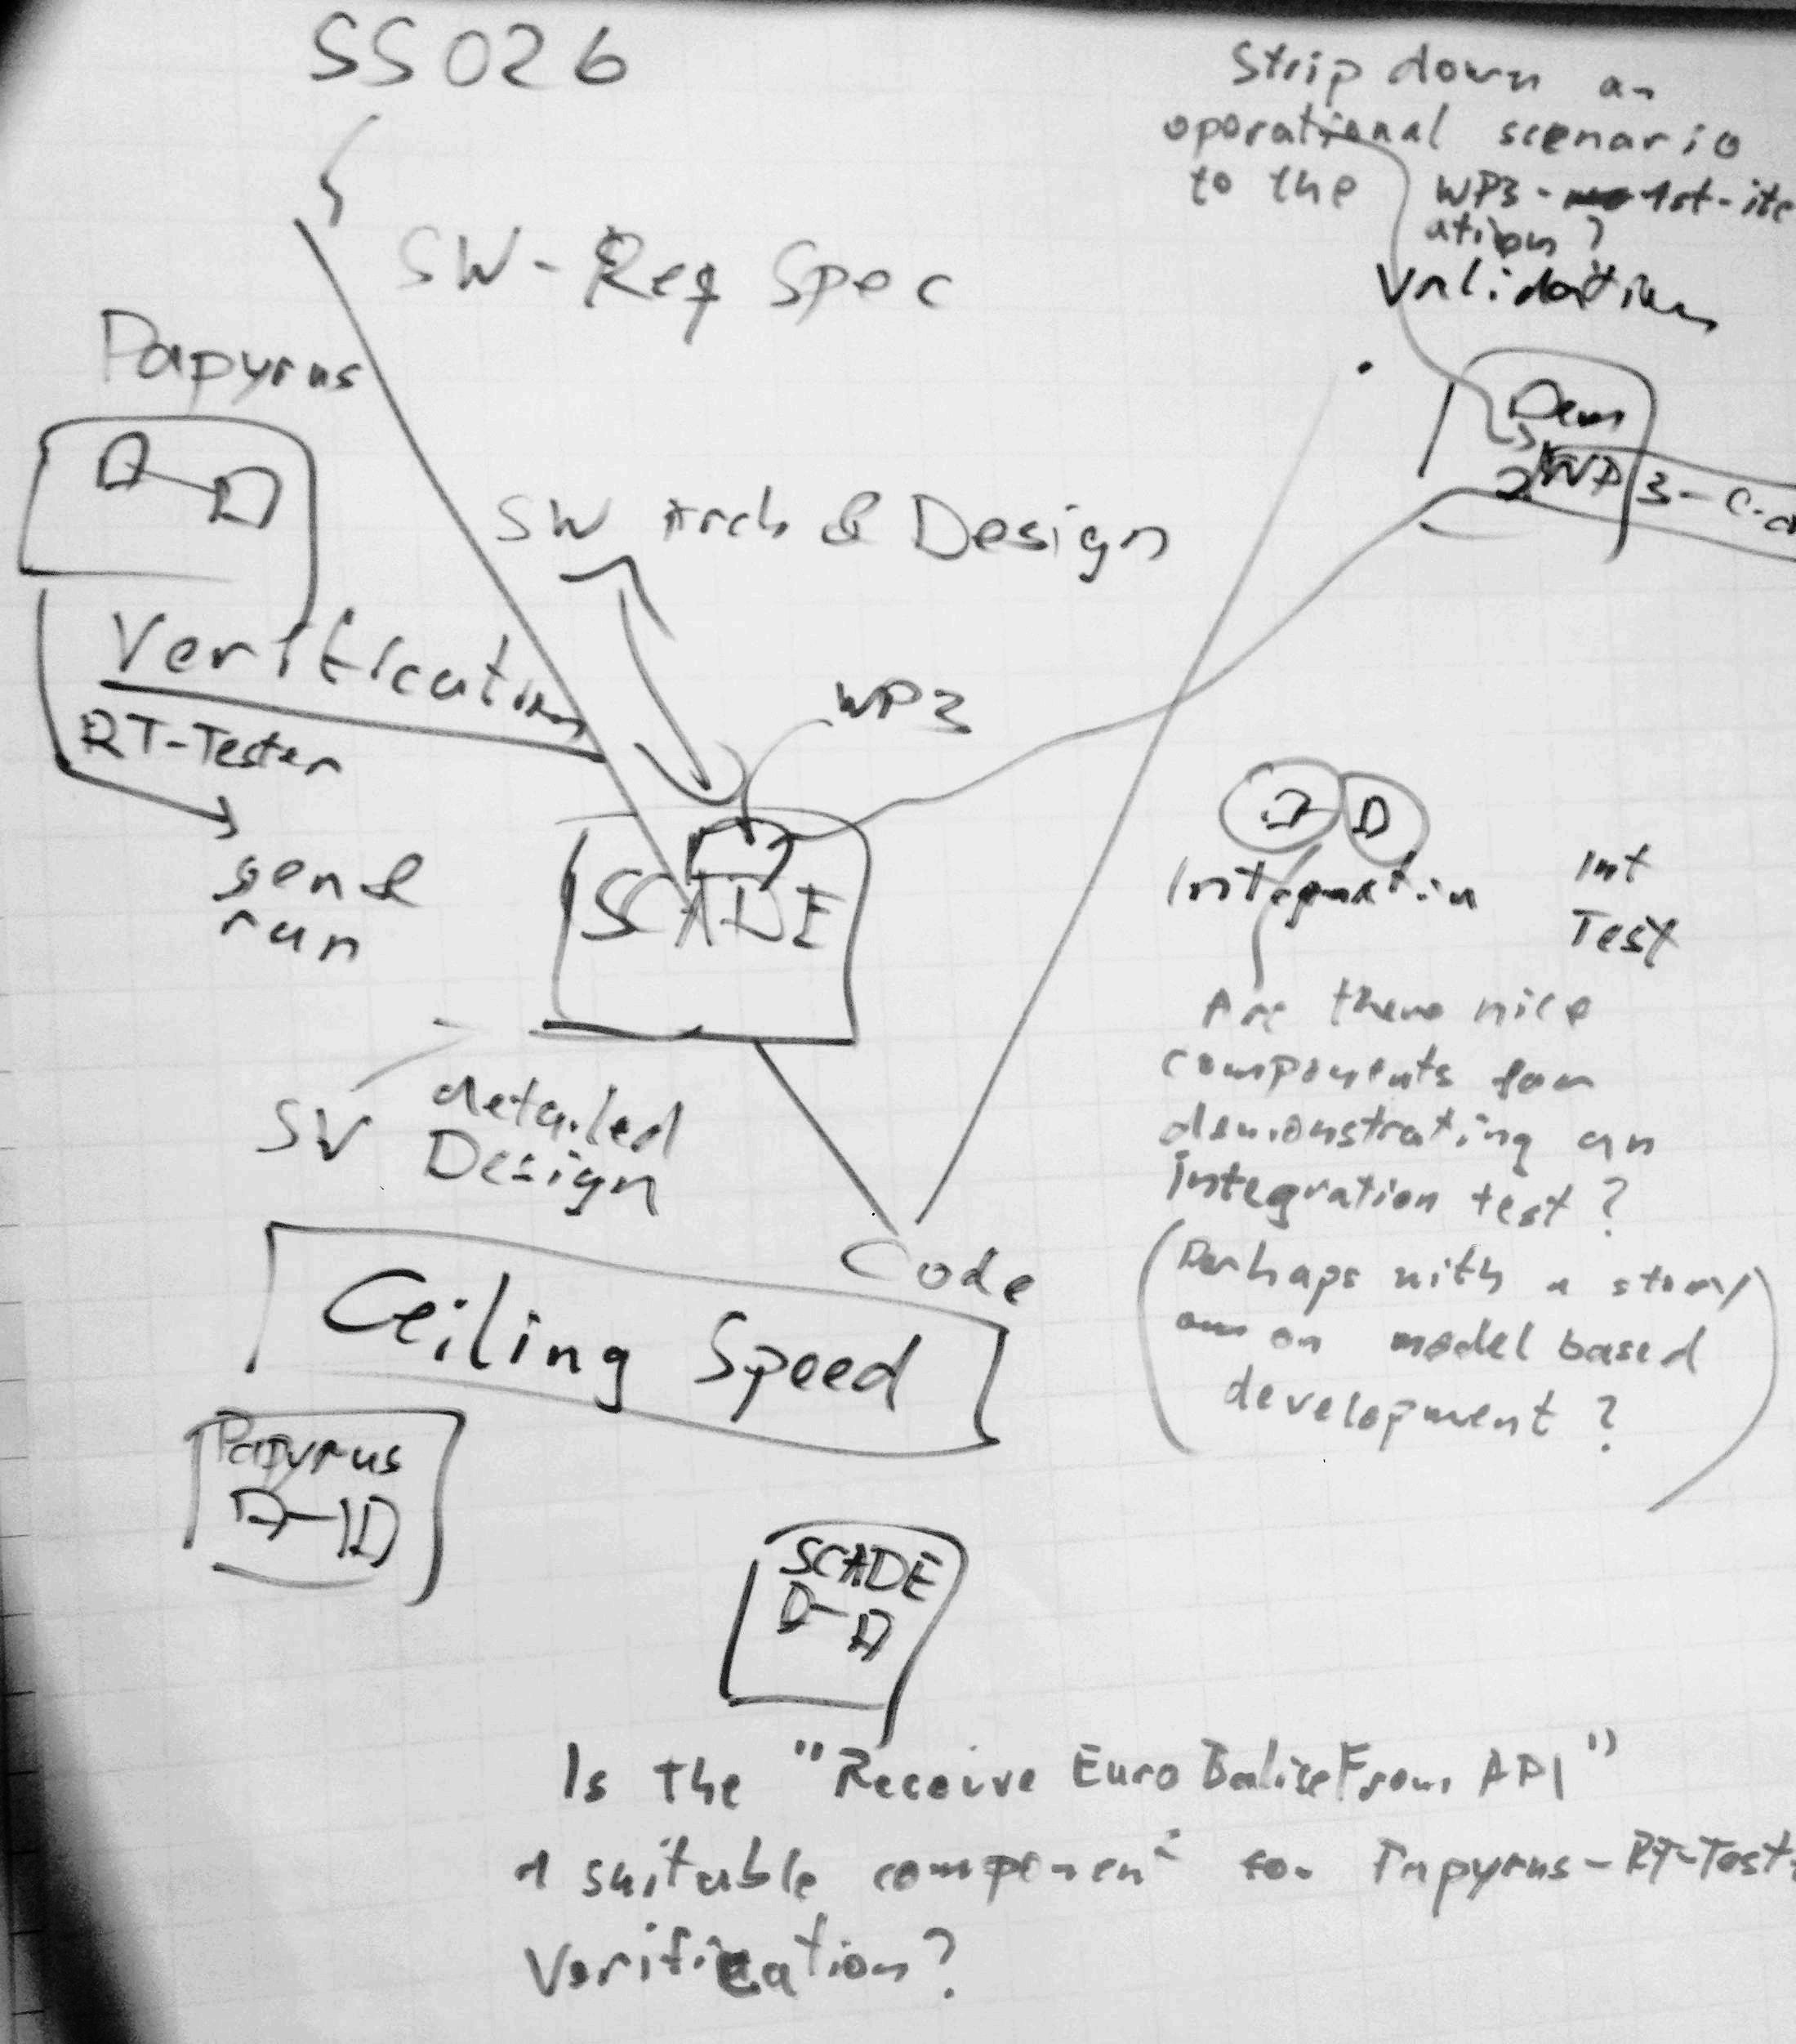
\includegraphics[height=125mm]{Sketch-C-crop-bw.jpg}
  \caption{Sketch of VnV demonstration wrt.\ development steps}
  \label{fig:sktchVnV}
\end{figure}

Three potential demonstrations of VnV. 
\begin{enumerate}
\item Verification of a \textbf{component}--- left side of the
  ``V''. For that, a Papyrus model of the component would be
  constructed, figuring as a part of the SW A\&D
  Specification. RT-Tester would be employed for test generation and
  execution. This parallels work done by the U Bremen on Ceiling Speed
  Monitoring. Tbd by DLR with support from U Bremen. Perhaps (who can
  give a hint?) the component ``ReceiveEuroBaliseFromAPI'' can be
  taken here.
\item Integration test of two (or more) \textbf{components}---middle
  of the right side of the ``V''. Two \textbf{components} which
  collaborate somehow are taken, and a function which employs both is
  tested. This is an instance of a standard integration
  test. Necessary (EN~50128), but nothing particular of openETCS
  methods in it. Here, the code generated from the components will
  stand for \textit{implementation code} (previous scenario: detailed design).
\item Validation demonstration---top right of the ``V''. According to
  the EN~50128, this takes place after SW/HW integration, perhaps
  partly with emulated HW. As long as there is no demonstrator
  incoporating the \textbf{release}, this cannot really be done. But one
  may demonstrate what would happen: Rephrasing an
  operational/functional scenario to what will happen at the interface
  of the \textbf{release} may show the contribution of the
  \textbf{release} (again, the code generated from it acts as
  implementation) to the validation.
\end{enumerate}

\eod


 

\end{document}